\pagebreak
\section{Algorithm Design}
\label{sec:algorithm}

\subsection{Taxi Allocation Daemon}
In this chapter there are some of the useful algorithms used in this project.
The first one is the taxi allocation daemon which receives 
new taxi requests and allocates a TaxiHandler for each request.

\lstset{
language=Java,
numbersep=10pt,
numbers=left,
frame=single,
}
\begin{lstlisting}[caption={Taxi allocation daemon}]
@Startup
@Singleton
class TaxiAllocationDaemon {
    /** Available taxis */
    private Map<Zone, LinkedList<Taxi>> taxis;

    /** A blocking queue containing new rides */
    private LinkedBlockingQueue<Ride> rides;

    /** ----- Class Methods ----- */

    /** Class constructor */
    public TaxiAllocationDaemon () { 
        /** Move arguments to class variables */
        taxis = new HashMap<Zone, LinkedList<Taxi>>();
        rides = new LinkedBlockingQueue<Ride>();
    }

    /** Main function */
    @PostConstruct
    public void run(){
        /** Keep looping while system is running */
        while( true ) {
            /** Get the next ride.(Blocking call) */
            Ride ride = rides.take();

            /** Get the associated zone */
            Zone zone = ride.getZone();

            /** Create and launch a TaxiHandler */
            new TaxiHandler(taxis.get(zone), ride)
                .start(); 
        }
    }

    /** Add a taxi to the specified zone queue */
    public void addTaxiToZoneQueue(
        Taxi taxi, Zone zone) {
        LinkedList<Taxi> list = taxis.get(zone);

        list.add(taxi);
    }

    /** This method is called when a new ride
     * is ready to be served */
    private void handleNewRide(Ride ride) {
        rides.add(ride);
    }

    /** This method is called every minute */
    @Schedule(minute="*")
    private void refreshRideQueue() {
        // (...) 
        if( newRideAvailable ) {
            handleNewRide(ride);
        }
    }
}
\end{lstlisting}
\pagebreak

\subsection{TaxiHandler}
This code is needed to find a suitable taxi for the designated ride.

\begin{lstlisting}[caption={TaxiHandler}]
class TaxiHandler extends Thread {
    private List<Taxi> taxis;
    private Ride ride;

    public TaxiHandler(LinkedList<Taxi> taxis, 
        Ride ride) {
        this.ride = ride;
        this.taxis = taxis;
    }

    @Override
    public void run() {
        selectTaxi();
    }

    private void selectTaxi() {
        /** Get the number of passengers */
        int nrPeople = ride.getNumberOfPassengers();
        PaymentMethod method = ride.getPaymentMethod();
        Taxi designatedTaxi = null;

        while( designatedTaxi == null ) {

            /** Find a valid taxi */
            for(Taxi taxi : taxis) {
                if( taxi.availableSeats() >= nrPeople 
                    && taxi.getPaymentMethods().
                        contains(method) 
                ){
                    designatedTaxi = taxi;
                    break;
                }
            }

            /** No taxi available */
            if(designatedTaxi == null) {
                throw 
                    new AgainstAssumptionsException();
            }

            if(!sendNotificationToTaxi(
                designatedTaxi)) {

                /** Re-enqueue taxi */
                taxis.remove(taxi);
                taxis.add(taxi);
                
                /** Choose another taxi */
                designatedTaxi = null;
            }
        }

        /** Bind the taxi with the ride */
        bindTaxi(designatedTaxi, ride);

        /** This taxi is now busy. */
        taxis.remove(designatedTaxi);
    }

    // (...)
}
\end{lstlisting}
\pagebreak


\subsection{Process call algorithm}
This algorithm is needed to process a call and add that in a suitable ride.
It takes as input parameter the call and returns the associated ride.

\begin{lstlisting}[caption={processCall()}]
public Ride processCall(Call call) {
    /** Is this call is a shareable reservation? */
    if(call instanceof Reservation && 
        ((Reservation)call).isShareable() {

        /** Get call parameters, 
         *  used to lookup active rides */
        Address startPoint = call.getStartPoint();
        Address endPoint = call.getEndPoint();
        int nrPeople = call.getNrPeople();

        /** Find a suitable ride */
        Ride ride = lookupSharedRide(
            startPoint, 
            endPoint, 
            nrPeople
        );

        /** There is a suitable shared ride. */
        if(ride != null) {
            ride.addCall(call);
            return ride;
        }
        
        /** Otherwise, create a new shared ride */
        return createSharedRide(call);
    } else {
        /** This call is not shareable. 
         *  Let's create a new normal ride
         */
        return createNormalRide(call); 
    }
}
\end{lstlisting}
\pagebreak
\subsection{Divide fees}
This is a quite simple algorithm used to divide the fee between 
people who are joining the ride. We decided to equally divide the fee
because even if the first customer would have to pay some extra route
in order to reach others, everyone starts from the same area; this means
that $C1_{C2} << C1_D$ and $C1_D \simeq C2_D$, where $X_Y$ is the cost of reaching Y from X. This implies that
\begin{equation}
    C1_D >> \frac{C1_{C2} + C2_D}{2}
\end{equation}

\begin{figure}[h!]
    \centering
    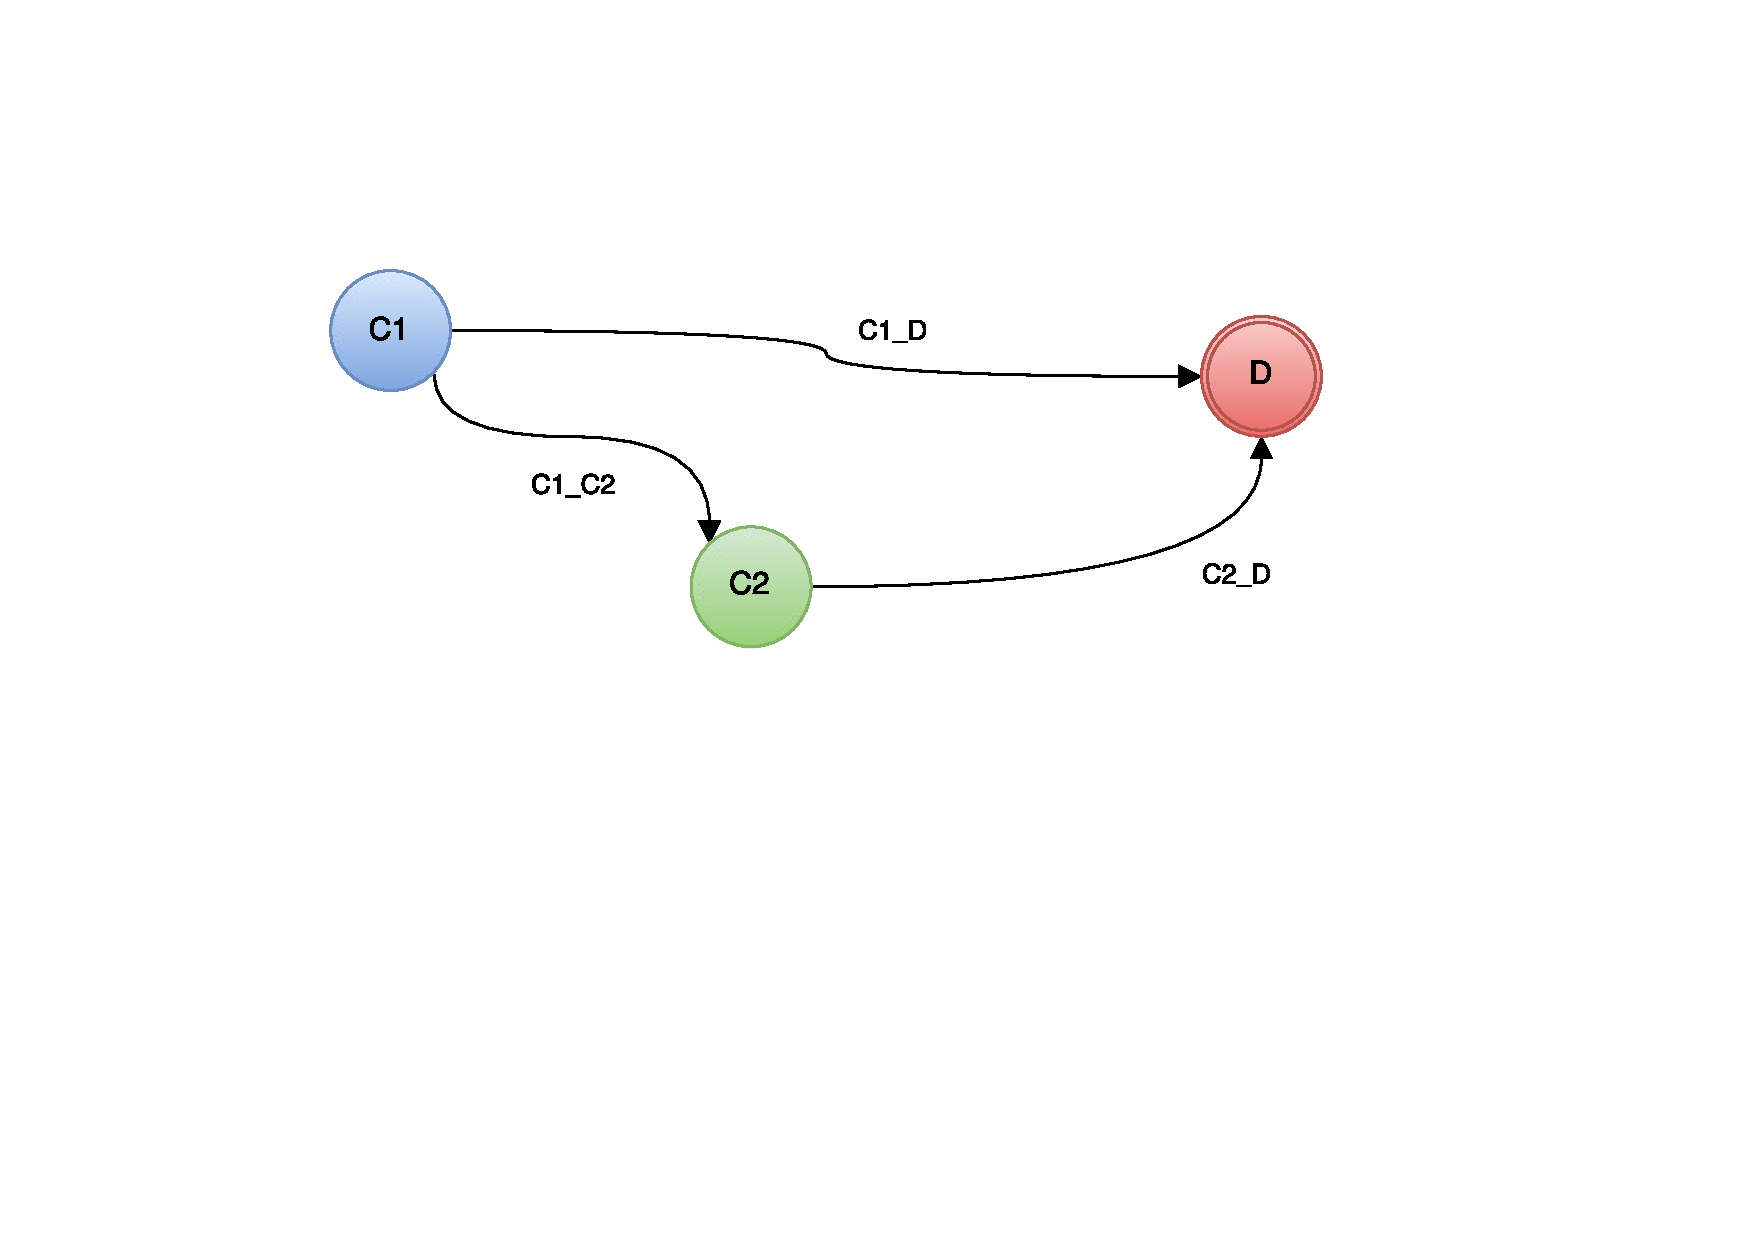
\includegraphics[width=0.9\textwidth]{Fee}
\end{figure}

Be careful, a check about $ nrPeople > 0 $ is needed in order to prevent
a division by zero.

\begin{lstlisting}[caption={Divide fees between partecipants}]
public void divideFees(double totalFee, int nrPeople) {
    if(nrPeople < 1)
        throw new InvalidNumberOfPeopleException();

    return totalFee / nrPeople;
}
\end{lstlisting}
